\documentclass[a4paper]{article}
\usepackage[english]{babel}
\usepackage[utf8]{inputenc}
\usepackage{graphicx}
\usepackage{enumitem}
\usepackage{blindtext}

\usepackage{amsfonts}
\usepackage{mathabx}

\graphicspath{ {./images/} }


\title{CS2200 Homework 3}
\author{Evan Wilcox}
\setlength\parindent{0pt}

\date{Due Feburary 26, 2019}

\begin{document}
  \maketitle

  \begin{enumerate}

    \item Fully recursive merge sort implemented in Python 2.7. 
    
    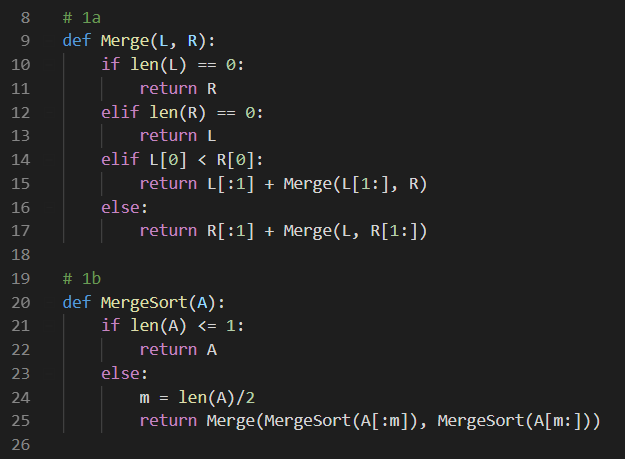
\includegraphics[scale=0.7]{1} \\



    \newpage
    \item Define an operation $\dotdiv$ called \textit{bounded subtraction} as follows:

    \begin{enumerate}
      \item $0 \dotdiv a = 0$
      \item $a \dotdiv 0 = a$
      \item $a' \dotdiv b' = a \dotdiv b$
    \end{enumerate}

    Prove that for all a, b in N, $(a+b) \dotdiv b = a$. \\

    Let $Q = \{q \in \mathbb{N} \: | \: (a+q) \dotdiv q = a \}$ \\
    $Q$ is not empty, $0 \in Q$ because $(a+0) \dotdiv 0 = a $
    
    
    \begin{tabular}{ |c|c|c| } \hline
      Start               & Current              & Reason                  \\ \hline
      $(a+q') \dotdiv q'$ & $=(a+q)' \dotdiv q'$ & Definition of +         \\ \hline
                          & $=(a+q) \dotdiv q$   & Definition of $\dotdiv$ \\ \hline
                          & $=a$                 & $q \in Q$               \\ \hline

    \end{tabular}


    \vspace{2cm}

    
    \item Simulator built in Python 2.7 that was used to test the .fsa files for problems 4 and 5. 
    
    A lines contain an A followed by a space followed by a string containing all the 
    characters in the alphabet. There can only be one A line.

    S lines contain an S followed by a space followed by the name of a state followed 
    by a comma and a space followed by a 0 or 1 if the state is a final state.

    B lines contain a B followed by a space followed by the name of the starting state. 
    There can only be one B line.

    D lines contain a D followed by a space followed by a state followed by a comma and
    a space followed by a character in the alphabet followed by a comma and a space
    followed by the next state.

    T lines contain a T followed by a space followed by the tape to be tested.

    O lines contain an O followed by a space. O lines must come directly after T lines.

    Lines must come in the order described above.

    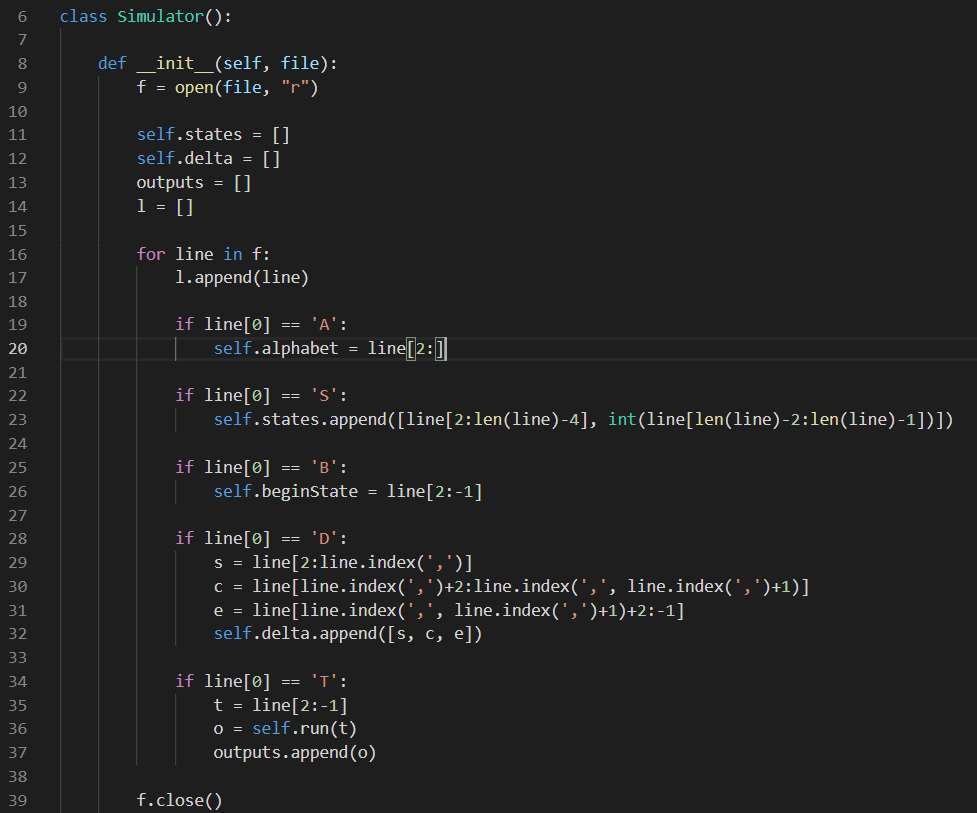
\includegraphics[scale=0.6]{3a} 
    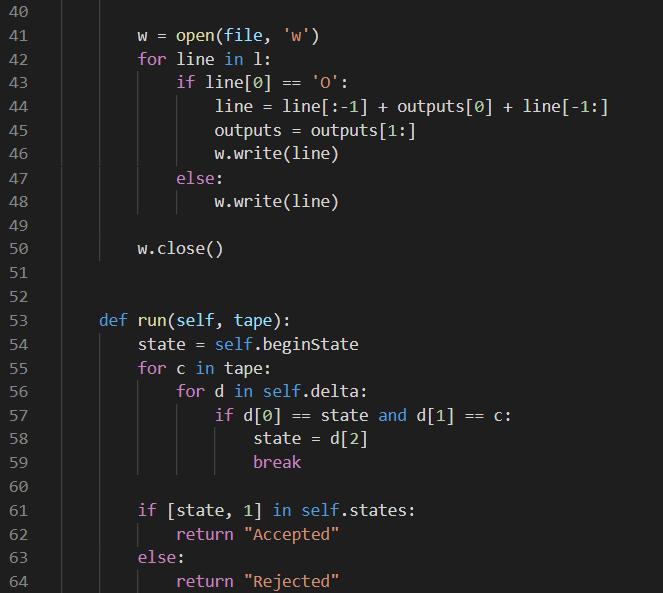
\includegraphics[scale=0.6]{3b}

    \newpage
    \item Find a deterministic finite-state automaton that recognizes the language, 
    L, consisting of all strings in \{a, b\}* that contain an odd number of b’s
    such that there is at least one “a” between every two b’s in the string. 
    \begin{center}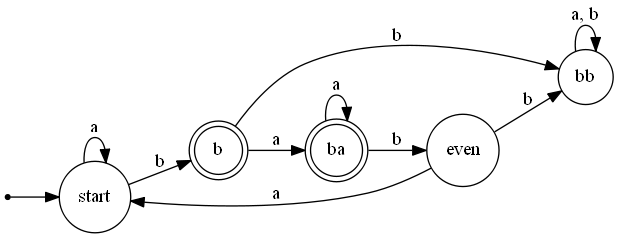
\includegraphics[scale=0.4]{4}\end{center}

    \begin{verbatim}
  A ab
  S start, 0
  S b, 1
  S ba, 1
  S bb, 0
  S even, 0
  B start
  D start, a, start
  D start, b, b
  D b, a, ba
  D b, b, bb
  D bb, a, bb
  D bb, b, bb
  D ba, a, ba
  D ba, b, even
  D even, a, start
  D even, b, bb
  T a
  O Rejected
  T b
  O Accepted
  T ab
  O Accepted
  T ba
  O Accepted
  T aba
  O Accepted
  T bab
  O Rejected
  T abaaaaba
  O Rejected
  T baaaaababa
  O Accepted
  T bb
  O Rejected
  T abbabbaba
  O Rejected
    \end{verbatim}


    \item Let L be a language over the alphabet \{d, e\} be the language of all
    strings having length $\leq$ 6. Construct a deterministic finite-state machine that
    recognizes L.
    \begin{center}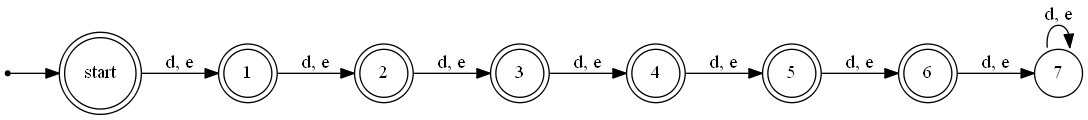
\includegraphics[scale=0.33]{5}\end{center}
    \begin{verbatim}
  A de
  S start, 1
  S 1, 1
  S 2, 1
  S 3, 1
  S 4, 1
  S 5, 1
  S 6, 1
  S 7, 0
  B start
  D start, d, 1
  D start, e, 1
  D 1, d, 2
  D 1, e, 2
  D 2, d, 3
  D 2, e, 3
  D 3, d, 4
  D 3, e, 4
  D 4, d, 5
  D 4, e, 5
  D 5, d, 6
  D 5, e, 6
  D 6, d, 7
  D 6, e, 7
  T 
  O Accepted
  T d
  O Accepted
  T e
  O Accepted
  T dd
  O Accepted
  T ee
  O Accepted
  T dedede
  O Accepted
  T ededed
  O Accepted
  T eeeeee
  O Accepted
  T dddddd
  O Accepted
  T eeeeeddddd
  O Rejected
  T ddedeeddeed
  O Rejected
      
    \end{verbatim}


  \end{enumerate}


\end{document}